Now let us create a general-purpose computer function for 
the purpose of $1D$ numerical advection of any given $1D$ 
function $q(x, t)$ (represented as a $1D$ array $q^n_i$) 
for any given velocity (also represented as a $1D$ array 
$v_{i+1/2}$). The function should receive the current
values of $q^n_i$, the velocities $v_{i+1/2}$ and a time 
step size $\Delta t$. It should return the values 
$q^{n+1}_i$, i.e. the values of $q$ at the next time step. 
For example, the function call in Python could look like 
qnew=advect(qold,vold,dx,dt), which advects $q^n_i$ one 
time step. Use ghost cells to implement the boundary 
conditions. \\
\\
You will use this function next week to create 
a general $1D$ hydrodynamics code from that, so please test 
this function and make sure that it works correctly. \\
\\
Note that the velocities $v_{i+1/2}$ are located in between 
the grid points. In the picture of grid cells: the 
velocities $v_{i+1/2}$ are defined on the cell boundaries 
while the to-be-advected function values $q^n_i$ are 
located in the cell centers. That also means that the 
length of the velocity array differs by one from the 
length of the $q$ array.

\paragraph{8. Apply your function to exercise 1.1 above 
    (with a constant velocity $v=1$) and convince yourself 
    that your function reproduces the same results.
} \ \\
    \\
    \lstinputlisting[firstline=4,lastline=21]{../code/ex2.py}


\paragraph{9. Now let us choose the velocity $v(x)=-2x/L$. 
    This is a converging velocity field. Take as an initial 
    density profile $q(x, 0)=1$ for $|x|\le L/4$ and 
    $q(x,0)=0$ for $|x|>L/4$. Integrate again in time from 
    $t=0$ to $t=3$ with 100 time steps. Plot the result at 
    different times and explain the result.
} \ \\
    \\
    \begin{figure}[h!]
        \centering
        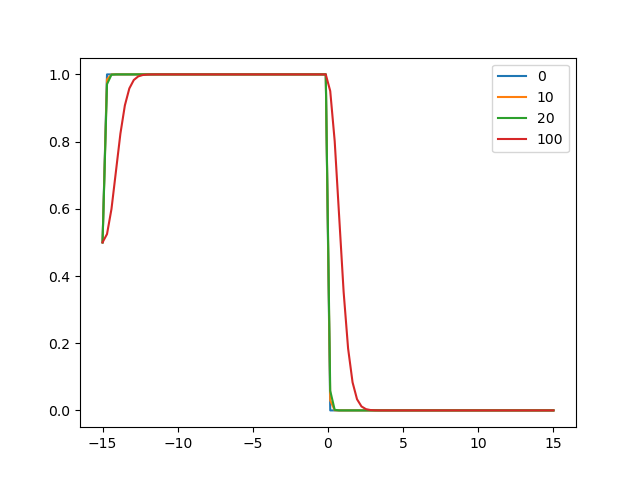
\includegraphics[width=\textwidth]{../figures/2.png}
        \caption{}
    \end{figure} \ \\ 
